\documentclass[a4paper,12p]{article}
\usepackage{standalone}
\usepackage{polski}
\usepackage[utf8]{inputenc}
\usepackage{amsmath}
\usepackage{physics}
\usepackage{amsfonts}
\usepackage{mathtools}
\usepackage{algorithm}% http://ctan.org/pkg/algorithms
\usepackage{algpseudocode}% http://ctan.org/pkg/algorithmicx
\usepackage{tikz}
\usepackage{amssymb}
\usepackage{indentfirst}
\usepackage{amsthm}
\usepackage{hyperref}
\linespread{1.5}

\renewcommand{\refname}{Źródła}
\newcommand\tab[1][1cm]{\hspace*{#1}}

\begin{document}

\begin{titlepage}
	\begin{center}
	
	{\huge\bfseries Algorytmy zaawansowane - projekt\par}
	\vspace{1cm}
	{\Large\scshape Wiktor Gontarczyk\par}
	{\Large\scshape Tomasz Laskowski\par}
	\vspace{2cm}

	\today
	\vspace{1cm}	
	
	\end{center}
\end{titlepage}

\tableofcontents

\newpage

\section{Cel projektu}

Celem projektu jest zaproponowanie algorytmu pozwalającego na wygenerowanie drzewa na podstawie macierz odległości pomiędzy liśćmi.


\section{Przedstawienie problemu}

Rozpatrzmy kwadratową, symetryczną macierz $D=[d_{ij}]_{n \times n}$ o wyrazach naturalnych. 

Problem $P$ o rozmiarze $n$ dla macierzy $D$ definiujemy jako zadania znalezienia (zbudowania) grafu nieskierowanego $G$ o zbiorze wierzchołków $V = l_1, l_2, \cdots l_n, v_{1}, \cdots, v{k}$ i zbiorze krawędzi $E \in (V \times V)^{n+k-1}$, t. że graf $G$ jest drzewem, wierzchołki $l_1, l_2, \cdots l_n$ są liśćmi tego drzewa oraz dla każdej pary liści $l_i, l_j \in V$, długość ścieżki pomiędzy nimi wynosi $d_{ij}$.

\section{Kod Prüfera}

Dla $n \in \mathbb{N}, n > 3$, kod Prüfera jest ciągiem $n - 2$ liczb od $1$ do $n$.

Kodowaniem Prüfera będziemy nazywać algorytm przyjmujący na wejściu drzewo $T$ o $n$ wierzchołkach i zwracający odpowiadający mu kod Prüfera. Zakładamy, że wierzchołki posiadają etykiety od $1$ do $n$.

\begin{algorithm}
		\floatname{algorithm}{Algorytm}
		\caption{Kodowanie Prüfera}
		\label{algo}
		$P$ = $\{ \}$ \\
		powtórz $n-2$ razy: \\
			\tab $v =$ liść o najniższej etykiecie w $T$ \\
			\tab dodaj do $P$ etykietę sąsiada $v$ \\
			\tab usuń $v$ z $T$ \\
		zwróć $P$
\end{algorithm}

Przykład dla $P = ( 3, 3, 4, 4 )$:

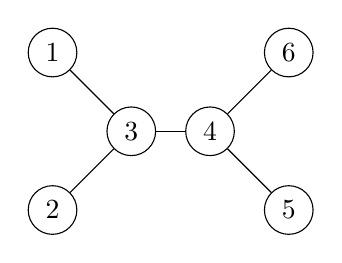
\begin{tikzpicture}
	\node[shape=circle,draw=black] (1) at (0,2) {1};
	\node[shape=circle,draw=black] (2) at (0,0) {2};
	\node[shape=circle,draw=black] (3) at (1,1) {3};
	\node[shape=circle,draw=black] (4) at (2,1) {4};
	\node[shape=circle,draw=black] (5) at (3,0) {5};
	\node[shape=circle,draw=black] (6) at (3,2) {6};
	
	\path [-] (1) edge node[left] {} (3);
	\path [-] (2) edge node[left] {} (3);
	\path [-] (3) edge node[left] {} (4);
	\path [-] (4) edge node[left] {} (5);
	\path [-] (4) edge node[left] {} (6);
\end{tikzpicture}

Dekodowaniem Prüfera nazywamy odwrotną operację tzn. otrzymanie kodu Prüfera odpowiadającego wejsciowemu drzewu $T$ o etykietowanych wierzchołkach. Przez $p_i$ będziemy oznaczać $i$-ty element kodu Prüfera $P$.

\begin{algorithm}
		\floatname{algorithm}{Algorytm}
		\caption{Dekodowanie Prüfera}
		\label{algo}
		
		$n = |P| + 2$ \\
		$V = \{ 1, 2, \cdots n \}$ \\
		$T = $ graf o $n$ wierzchołkach bez krawędzi \\
		dla $i$ od $1$ do $n-2$: \\
			\tab $v =$ wierzchołek o etykiecie będącej najmniejszą wartością z $V$, którego nie ma w $P$ \\
			\tab dodaj do $T$ krawędź z $v$ do wierzchołka o etykiecie $p_i$ \\
			\tab usuń $v$ z $V$ \\
			\tab usuń $p_i$ z $P$ \\
		dodaj do $T$ krawędź pomiędzy dwoma wierzchołkami o etykietach z pozostałych elementów $V$ \Comment{Zawsze zostaną dwa elementy}
\end{algorithm}

Przykład: \\
$E=\{\},~P=(3,3,4,4),~V=(1,2,3,4,5,6)$ \\
$E=\{(1,3)\},~P=(3,4,4),~V=(2,3,4,5,6)$ \\
$E=\{(1,3), (2,3)\},~P=(4,4),~V=(3,4,5,6)$ \\
$E=\{(1,3), (2,3), (3,4)\},~P=(4),~V=(4,5,6)$ \\
$E=\{(1,3), (2,3), (3,4), (4,5)\},~P=\{\},~V=(4,6)$ \\
$E=\{(1,3), (2,3), (3,4), (4,5), (4,6)\},~P=\{\},~V=\{\}$ \\

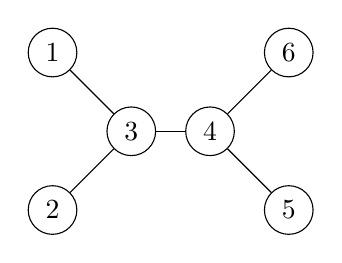
\begin{tikzpicture}
	\node[shape=circle,draw=black] (1) at (0,2) {1};
	\node[shape=circle,draw=black] (2) at (0,0) {2};
	\node[shape=circle,draw=black] (3) at (1,1) {3};
	\node[shape=circle,draw=black] (4) at (2,1) {4};
	\node[shape=circle,draw=black] (5) at (3,0) {5};
	\node[shape=circle,draw=black] (6) at (3,2) {6};
	
	\path [-] (1) edge node[left] {} (3);
	\path [-] (2) edge node[left] {} (3);
	\path [-] (3) edge node[left] {} (4);
	\path [-] (4) edge node[left] {} (5);
	\path [-] (4) edge node[left] {} (6);
\end{tikzpicture}

\newpage

\section{Format wejścia i wyjścia}

Algorytm przyjmuje dwa argumenty: zbiór etykiet liści $R$ oraz macierz odległości $D$. Macierz ta musi spełniać trzy warunki:

\begin{itemize}
	\item musi być symetryczna
	\item na diagonali muszą się znajdować zera
	\item jej kolumny i wiersze powinny być etykietowane liczbami naturalnymi (odpowiadającymi wierzchołkom grafu), zbiór etykiet powinien się pokrywać ze zbiorem $R$ 
\end{itemize}

Macierz odległości $D$ w implementacji musi być reprezentowana jako dwuwymiarowa tablica z możliwością etykietowania kolumn/wiersz (np. ramka danych). Program implementujący algorytm będzie również musiał dokonać walidacji wymienionych wcześniej warunków.

Algorytm zwraca sekwencję $P$, reprezentującą kod Prüfera, który jednoznacznie reprezentuje graf (poprzedni rozdział).

\newpage

\section{Pseudokod algorytmu}

\begin{algorithm}
		\floatname{algorithm}{Algorytm}
		\caption{Główny algorytm}
		\label{algo}
		\textbf{repeat} \\
		\tab  $S = \{ \}$ \\
		\tab \textbf{while} (R jest niepusty) \\
		\tab \tab $k$ = liść z najniższą etykietą w $R$ \\
		\tab \tab \textbf{if} $k$ ma w $P$ sąsiada $P_i$ \\
		\tab \tab \tab $m = P_i$ \\
		\tab \tab \tab dodaj $m$ do $P$ \\
		\tab \tab \tab Usuń $k$ z $R$ \\
		\tab \tab \tab Usuń $k$ z $D$ \\
		\tab \tab \tab \textbf{if} w $D$ nie ma już wierzchołków
		\tab \tab \tab przerwij główną pętlę
		\tab \tab \textbf{else} \\
		\tab \tab \tab $lastNode = lastNode + 1$ \\
		\tab \tab \tab $m = lastNode$ \\
		\tab \tab \tab dodaj $m$ do $P$ \\
		\tab \tab \tab Usuń $k$ z $R$ \\
		\tab \tab \tab Usuń $k$ z $D$ \\
		\tab \tab \tab $d_{im} = d_{mi} = d_{ik} - 1$, dla $i = 1, 2, \cdots m-1$ \\
		\tab \tab \tab dodaj $m$ do $S$ \\
		\tab  $R'$ = getleaves(S, D) \\
		\tab \textbf{if} $|R'| == 2$ i $d_{ij} == 1$ \\
		\tab \tab return $P$ \\
		\tab \textbf{else} \\
		\tab \tab $R = R'$ \\
		\textbf{return} $P$ \\
\end{algorithm}

W pseudokodzie użyta została funkcja getleaves, której zadaniem jest wybranie zbioru liści ze zbioru wierzchołków - ozn. $S$ w pseudokodzie.

Funkcja przyjmuje zbiór wierzchołków $S$ o etykietach od $1$ do $|S|$ i macierz odległości $D$, zwraca zbiór wierzchołków, będących liśćmi w zbiorze $S$.

\begin{algorithm}
		\floatname{algorithm}{Algorytm}
		\caption{Funkcja getleaves}
		\label{algo}
		oznacz wszystkie wierzchołki $S$ jako liście \\
		\textbf{for} i \textbf{in} $1, \cdots |S|$ \\
		\tab \textbf{for} j \textbf{in} $1, \cdots |S|$ \\
		\tab \tab \textbf{for} i \textbf{in} $1, \cdots |S|$ \\
		\tab \tab \tab \textbf{if} $d_{ij} = d_{ik} + d+k$ \\
		\tab \tab \tab \tab oznacz wierzchołek z etykietą $k$ jako nie-liść \\
		\textbf{return} zbiór wierzchołków $S$ oznaczonych jako liście \\
\end{algorithm}

\section{Dowód poprawności}

Poprawność algorytmu opiera się na poprawności kodowania Prüfera i twierdzeniu, że algorytm wyznacza unikalny kod Prüfera dla danej macierzy wejściowej.

\newtheorem{lem}{Twierdzenie}

\begin{lem}
	Powyższy algorytm wyznacza unikalny kod Prüfera dla macierzy odległości $D_{ij}$.
\end{lem}

\begin{proof}
Niech $T = (V, E)$ będzie drzewem o $n$ wierzchołkach.
Niech $A$ będzie macierzą sąsiedztwa drzewa $T$, zdefiniowaną jako
\[
  A_{ij} = \left.
  \begin{cases}
    1, & \text{dla } (i, j) \in E \\
    0, & \text{dla } (i, j) \notin E
  \end{cases}
  \right.
\]

Niech R = {1, 2, 3, \dots, r}, będzie początkowym zbiorem liści. Oznaczmy zbiór wierzchołków wewnętrznych jako $K = \{m, m+1, m+2, \dots, m+k-1\}$, $m=r+1$ $|R| = r$ i $|K|=k$, $r \geq 2$, $k \geq 1$. Liczba wierzchołków drzewa $T$, wynosi $n = r + k$.
Przyjmijmy, że $P$ i $Q$ są dwoma różnymi kodami Prüfera o długości $n-2$ uzyskanymi przez zastosowanie algorytmu dla macierzy $D_{ij}$.
$P$ i $Q$ zawierają etykiety z K (liście nie występują w ciągu) i każdy wierzchołek z $K$ pojawia się w ciągu co najmniej raz.

Kody $P$ i $Q$ muszą się różnić na co najmniej jednej pozycji i dla dowolnej pary wierchołków istnieje unikalna ścieżka między nimi. Wystarczy więc pokazać, że jakakolwiek zmiana ciągu powoduje modyfikację macierzy sąsiedztwa i w rezultacie modyfikuje macierz odległości.

Niech $last_{1, \dots, n-2}$ będzie tablicą oznaczającą skrajnie prawe (ostatnie) wystąpienie etykiety w kodzie. Wartość $last_i = 1$, gdy $i$ jest skrajnie prawym indeksem w kodzie dla wierzchołka $P_i$ i 0 w przeciwnym przypadku.

Niech $R'$ będzie nowym zbiorem liści, po wyrzuceniu liści z poprzedniej iteracji. Zbiór ten tworzymy, poprzez dodanie $P_i$ do $R'$, gdy $last_i = 1$ dla poprzedniego ciągu.

Początkowo macierz sąsiedztwa $A{n \times n}$ jest wypełniona zerami. Element $A_{ij}$ przyjmuje wartość 1 w następujących przypadkach:

Gdy $i \in R$:
  Pierwsze r wierzchołków kodu Prüfera są incydentne z liśćmi z $R$.
  $A_{i, P_i} = 1, \text{dla } i = 1, 2, \dots, r$

Gdy $i \in K$:
  Rozważmy nowy zbiór liści $R'$ taki, że $2 \leq |R'| \leq |R|$ 
  $A_{ij} = 1$, gdy $ i \in R' $ i $j = P_t $, gdzie $P_t$ jest sąsiadem $i$ i $t$ oznacza indeks etykiety w kodzie Prüfera pomiędzy
   $|R| + 1$, a $|R| + |R'|$, tzn. $|R| < t \leq |R| + |R'|$.

Zbiór $R'$ jest wyznaczany w każdej iteracji algorytmu i powiększa zbiór $R$. Iteracje powtarzamy dopóki $R' \neq \O$.

Kody $P$ i $Q$ mogą różnić się w następujących przypadkach:

Przypadek I

Kody $P$ i $Q$ różnią się na pierwszych $r$ pozycjach. W takiej sytuacji liście będą miały inne sąsiedztwo i różne też będą macierze sąsiedztwa dla $P$ i $Q$.

Przypadek II

Kody $P$ i $Q$ różnią się na pozostałych k pozycjach. Wtedy zbiór $R'$ będzie różny dla obu kodów w co najmniej jednej iteracji i różne też będą wierzchołki sąsiadujące.

W obu przypadkach zmiana dowolnej wartości w kodzie skutkuje zmianą macierzy sąsiedztwa i w strukturze drzewa.

Zatem $P$ i $Q$ muszą być identyczne jeśli kodują drzewa o identycznych macierzach sąsiedztwa, co kończy dowód.
\end{proof}


\section{Złożoność obliczeniowa}

Załóżmy, że rozwiązujemy problem wielkości $n$, gdzie $n$ to liczba wierzchołków wejściowego zbioru liści. Na złożoność obliczeniową największy wpływ ma funkcja \texttt{getleaves} o złożoności $\mathcal{O}(n^3)$ - zawiera ona potrójną pętlę po wszystkich wierzchołkach zbioru tymczasowego, którego pesymistyczna wielkość wynosi $n$. Dodawanie wierzchołka do tymczasowego zbioru $S$ ma pesymistyczną złożoność $\mathcal{O}(n)$ - musimy przejrzeć pełną listę wierzchołków. To samo tyczy się operacji, wymagających przeszukiwania zbioru wierzchołków lub wiersz macierzy odległości. Reszta operacji wykonywana jest w czasie stałym.

Aby obliczyć pesymistyczną złożoność należy oszacować liczbę wykonań głównej pętli algorytmu. Posłużą nam do tego dwa spostrzeżenia o zmianach długości ścieżek podczas kolejnych iteracji. Po pierwsze należy zauważyć, że za każdym wykonaniem pętli usuwamy minimum $2$ liście z rozważań, co oznacza, że za każdą iteracją, długość każdej ze ścieżek zmniejsza się o $2$. Po drugie algorytm zatrzyma się i zwróci wynik, kiedy pozostaną tylko dwa liście i odległość między nimi będzie wynosić $1$. Zakładając, że maksymalna ścieżka w wejściowej macierzy odległości $D$ wyniesie $l_{max}$, pesymistyczna liczba wykonań głównej pętli wyniesie $\frac{l_{max}}{2}$. Złożoność obliczeniowa wyniesie $\mathcal{O}(\frac{l_{max}}{2} n^3)$. Okazuje się więc, że złożoność obliczeniowa algorytmu, zależy nie tylko od wejściowej wielkości problemu, ale i od maksymalnej długości ścieżki.

\newpage

\begin{thebibliography}{1}
\bibitem{TreeInference} C. Vanniarajan, Kamala Krithivasan, Network (Tree) Topology Inference Based on Prüfer Sequence, \url{http://www.cse.iitm.ac.in/~kamala/NCC2010_Topology_Inference_V1_1.pdf}
\end{thebibliography}

\end{document}